PanDA is a Workload Management System (WMS) %~\cite{marco2009glite} 
designed to support the execution of distributed workloads and workflows via
pilots~\cite{turilli2017comprehensive}. Pilot-capable WMS enable high
throughput execution of tasks via multi-level scheduling while supporting
interoperability across multiple sites. This is particularly relevant for LHC
experiments, where millions of tasks are executed across multiple sites every
month, analyzing and producing petabytes of data.

The implementation of PanDA WMS consists of several interconnected
subsystems, communicating via dedicated API or HTTP messaging, and
implemented by one or more modules. Databases are used to store stateful
entities like tasks, jobs and input/output data, and to store information
about sites, resources, logs, and accounting.

Currently, PanDA's architecture has five main subsystems: PanDA
Server~\cite{maeno2011overview},
AutoPyFactory~\cite{caballero2012autopyfactory}, PanDA
Pilot~\cite{nilsson2011atlas}, JEDI~\cite{borodin2015scaling}, and PanDA
Monitoring~\cite{klimentov2011atlas}. Other subsystems are used by some of
ATLAS workflows but we do not discuss them as they are not relevant to an
understanding of how PanDA has been ported to supercomputers. For a full list
of subsystems see Ref.~\cite{panda-wiki_url}. Fig.~\ref{fig:architecture}
shows a diagrammatic representation of PanDA main subsystems, highlighting
the execution process of tasks while omitting monitoring details to improve
readability.

Users submit task descriptions to JEDI (Fig.~\ref{fig:architecture}:1) that
stores them into a queue implemented by a database
(Fig.~\ref{fig:architecture}:2). Tasks are partitioned into jobs of different
size, depending on both static and dynamic information about available
resources (Fig.~\ref{fig:architecture}:3). Jobs are bound to sites with
resources that best match jobs' requirements, and submitted to the PanDA
Server for execution (Fig.~\ref{fig:architecture}:4).

Once submitted to the PanDA Server, jobs are stored by the Task Buffer
component into a global queue implemented as a database
(Fig.~\ref{fig:architecture}:5). When jobs are submitted directly to the
PanDA Server, the Brokerage component is used to bind jobs to available
sites, depending on static information about the resources available for each
site. Jobs submitted by JEDI are already bound to sites so no further
brokerage is needed.

Once jobs are bound to sites, the Brokerage module communicates to the Data
Service module what data sets need to be made available on what site
(Fig.~\ref{fig:architecture}:6). The Data Service communicates these
requirements to the ATLAS DDM (Fig.~\ref{fig:architecture}:7) that, when
needed, replicates data sets on the required sites
(Fig.~\ref{fig:architecture}:8).

Meanwhile, AutoPyFactory defines PanDA Pilots, submitting them to a Condor-G
agent (Fig.~\ref{fig:architecture}:9). Condor-G schedules these pilots
wrapped as jobs to the required sites (Fig.~\ref{fig:architecture}:10).

When a PanDA Pilot becomes available, it requests the Job Dispatcher module
of the PanDA Server for a job to execute (Fig.~\ref{fig:architecture}:11).
The Job Dispatcher interrogates the Task Buffer module for a job that is
bound to the site of that pilot and ready to be executed. Task Buffer checks
the global queue (i.e., the PanDA DB) and, upon availability, returns a job
to the Job Dispatcher. The Job Dispatcher dispatches that job to the PanDA
Pilot (Fig.~\ref{fig:architecture}:12).

Each PanDA Pilot starts a monitoring process on receiving a job and forks a
subprocess to execute the job's payload. Input data are transferred from the
stage-in location (Fig.~\ref{fig:architecture}:13), the job's payload is
executed (Fig.~\ref{fig:architecture}:14) and once completed, output is
transferred to the staging-out location (Fig.~\ref{fig:architecture}:15).

The Data Service module of the PanDA Server tracks and collects the output
generated by each job (Fig.~\ref{fig:architecture}:16), updating jobs'
attributes via the Task Buffer module (Fig.~\ref{fig:architecture}:17). When
the output of all the jobs of a task are retrieved, it is made available to
the user via PanDA Server. When a task is submitted to JEDI, task is instead
marked as done (Fig.~\ref{fig:architecture}:18) and the result of its
execution is made available to the user by JEDI
(Fig.~\ref{fig:architecture}:19).

\begin{figure}
    \centering
    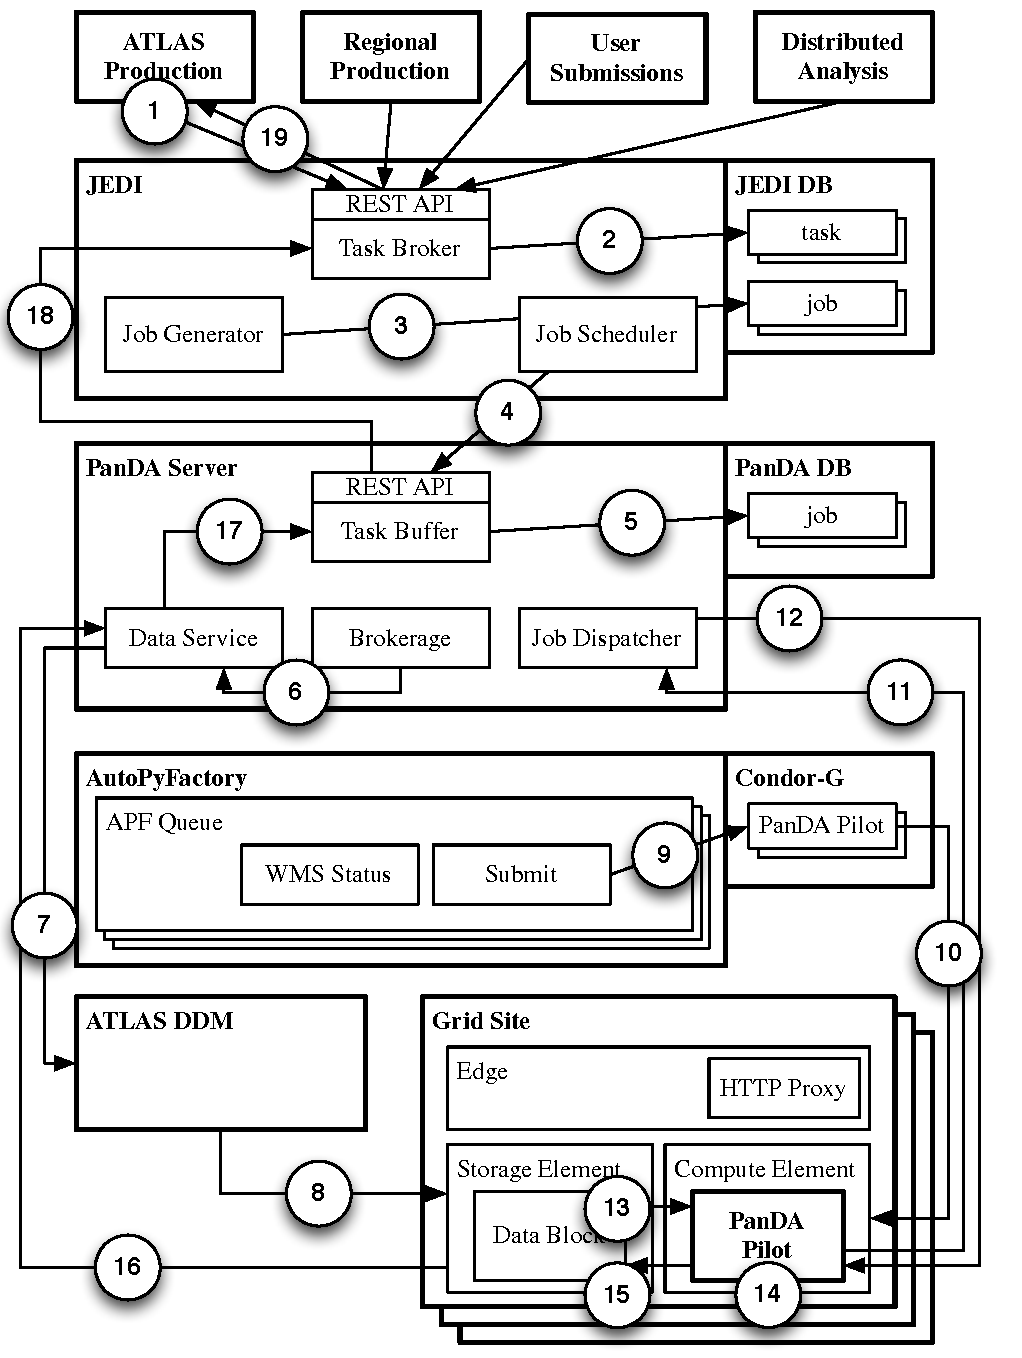
\includegraphics[width=\columnwidth]{panda_architecture.pdf}
    \vspace{-0.3in}
    \caption{PanDA WMS architecture. Numbers indicates the JEDI-based
    execution process described in \S\ref{sec:panda_overview}. Several
    subsystems, components, and architectural and communication details are
    abstracted to improve clarity.}\label{fig:architecture}
\end{figure}